
%(BEGIN_QUESTION)
% Copyright 2011, Tony R. Kuphaldt, released under the Creative Commons Attribution License (v 1.0)
% This means you may do almost anything with this work of mine, so long as you give me proper credit

A computer spreadsheet program may be used as a simulator for a {\it median select} function, choosing the median of three values input to it.

Begin creating your own spreadsheet by following the format shown below, allowing anyone to enter three values into cells on the left-hand side of the workbook, while the spreadsheet chooses and displays the median value in a cell toward the right-hand side of the workbook.  The yellow (input) and blue (output) cell shading is optional:

$$\includegraphics[width=15.5cm]{i00790x01.eps}$$

Where might a median-select function be used in a process control system?

\vskip 20pt \vbox{\hrule \hbox{\strut \vrule{} {\bf Suggestions for Socratic discussion} \vrule} \hrule}

\begin{itemize}
\item{} There is definitely more than one way to accomplish this function using a spreadsheet program.  Identify at least two of them.
\end{itemize}

\underbar{file i00790}
%(END_QUESTION)





%(BEGIN_ANSWER)


%(END_ANSWER)





%(BEGIN_NOTES)


%INDEX% Computer spreadsheet exercise: median-select function
%INDEX% Relay, computational: median select 

%(END_NOTES)

